\documentclass[11pt]{article}

\usepackage[margin=1in]{geometry}
\usepackage{amsmath,amssymb,amsfonts,bm}
\usepackage{graphicx}
\usepackage{xcolor}
\usepackage{float}
\usepackage{listings}
\usepackage{enumitem}
\usepackage{booktabs}
\usepackage{hyperref}
\usepackage{xurl}
\usepackage{fancyhdr}

\setkeys{Gin}{width=0.75\textwidth}
\setlength{\parindent}{0pt}
\Urlmuskip=0mu plus 1mu

% ---------- Header setup ----------
\pagestyle{fancy}
\fancyhf{}
\fancyhead[L]{\today}
\fancyhead[C]{Homework \#5}
\fancyhead[R]{Scott Nguyen}
\renewcommand{\headrulewidth}{0.4pt}
\fancyfoot[C]{\thepage}

\begin{document}
	
	\begin{center}
		{\Large Homework \#5: Distributions and Fourier Transforms: How to differentiate functions for Deep Learning, take Fourier Transforms of tempered distributions, and visualize convolutions in Neural Networks using Fourier Transforms}
		
		\vspace{0.5em}
		March 19, 2026
	\end{center}
	
	\textbf{Warning:} You are expected to provide answers in your own words based on the discussion held in class. You will receive no credit for copying material from an AI chatbot, the internet, or if your discussion simply does not reflect the class discussion of what is expected. The use of AI or online resources is not prohibited. However, you need to use your own words, and your answers need to align with class discussions.
	
	\hrule
	\vspace{1em}
	
	% ============================================================
	\textbf{Problem \#1. Differentiating Functions.}
	
	The most essential innovation of Deep Learning is to provide automated methods for the differentiation of functions. Once you have derivatives, you can optimize.
	
	This problem reviews differentiation in the context of distribution theory. In regular calculus, we note that continuity does not guarantee that we can differentiate. Using Distributions, we can differentiate discontinuous functions!
	
	In general, we defined derivatives using:
	\[
	\left\langle \frac{\partial f}{\partial x_k}, \phi \right\rangle
	= -
	\left\langle f, \frac{\partial \phi}{\partial x_k} \right\rangle.
	\]
	
	where:
	\[
	\left\langle f, \frac{\partial \phi}{\partial x_k} \right\rangle
	= -
	\int_{\mathbb{R}} f(x) \frac{\partial \phi(x)}{\partial x} dx
	\]
	
	and $\phi$ is a test function: $f \in D(\Omega)$ (see definition in the lecture notes).
	
	In the notes, we differentiated two functions that do not have derivatives in the ordinary sense:
	\[
	\frac{d u(t)}{dt} = \delta(t)
	\]
	\[
	\frac{d}{dx}\text{ReLU}(x) =
	\begin{cases}
		1, & x > 0 \\
		0, & x \le 0
	\end{cases}
	\]
	
	At the end of our lecture, we note that distribution derivatives coincide with regular derivatives when the function is continuous. Note that regular calculus also requires differentiability. We can use our regular calculus understanding here because $\phi$ is assumed to have derivatives of all orders everywhere.
	
	In this problem, we aim to show that moving the ReLU around, as is often done in Neural Networks, yields the expected results. The same applies to the step function.
	
	Follow the same process as in the lecture notes to show that:
	\[
	\frac{d}{dx}\text{ReLU}(x - 5) =
	\begin{cases}
		1, & x > 5 \\
		0, & x \le 5
	\end{cases}
	\]
	
	Follow the same steps as for ReLU(x) provided in the lecture notes.
	
	Note that translation simply translates the derivative!\\
	
	\textbf{Solution.}
	Define
	\[
	g(x)=\mathrm{ReLU}(x-5)=
	\begin{cases}
		x-5, & x>5,\\
		0, & x\le 5.
	\end{cases}
	\]
	We use the distribution derivative definition:
	\[
	\left\langle \frac{d g}{dx}, \phi \right\rangle
	=
	-
	\left\langle g,\frac{d\phi}{dx}\right\rangle.
	\]
	
	Step 1. Evaluate the RHS:
	\[
	\left\langle \frac{d g}{dx}, \phi \right\rangle
	=
	-\int_{-\infty}^{\infty} \mathrm{ReLU}(x-5)\,\phi'(x)\,dx
	=
	-\int_{5}^{\infty} (x-5)\phi'(x)\,dx.
	\]
	Apply integration by parts:
	\[
	\int_{5}^{\infty} (x-5)\phi'(x)\,dx
	=
	(x-5)\phi(x)\Big|_{5}^{\infty}
	-
	\int_{5}^{\infty}\phi(x)\,dx.
	\]
	Since \(\phi\) is a test function, \(\phi(\infty)=0\), and since \(x-5=0\) at \(x=5\), the boundary term is zero. Thus,
	\[
	\int_{5}^{\infty} (x-5)\phi'(x)\,dx
	=
	-\int_{5}^{\infty}\phi(x)\,dx.
	\]
	Therefore,
	\[
	\left\langle \frac{d g}{dx}, \phi \right\rangle
	=
	\int_{5}^{\infty}\phi(x)\,dx.
	\]
	
	Step 2. Guess a function for the derivative:
	\[
	\psi(x)=
	\begin{cases}
		1, & x>5,\\
		0, & x\le 5.
	\end{cases}
	\]
	Then, as a distribution,
	\[
	\langle \psi,\phi\rangle
	=
	\int_{5}^{\infty}\phi(x)\,dx.
	\]
	
	Step 3. Compare both sides.
	
	Both \(\dfrac{d}{dx}\mathrm{ReLU}(x-5)\) and \(\psi(x)\) give the same action on every test function \(\phi\). Hence,
	\[
	\frac{d}{dx}\mathrm{ReLU}(x-5)
	=
	\begin{cases}
		1, & x>5,\\
		0, & x\le 5.
	\end{cases}
	\]
	
	Thus, translation simply translates the derivative.
	
	\newpage
	
	% ============================================================
	\textbf{Problem \#2. Fourier Transforms for Tempered Distributions}
	
	\vspace{0.5em}
	
	\textbf{2(a)} Suppose that we want to evaluate the Fourier Transform of $exp(j\omega_0 x)$ where $\omega_0$ is a constant ($\omega$ instead of $\xi$ here!). We begin by establishing the need for a new theory! Show that the following integral is not well defined:
	\[
	\hat{g}(\omega) = \int_{\mathbb{R}} exp(j\omega_0 x) exp(j\omega x) dx.
	\]
	
	To show that this is not well defined, follow the steps below:
	
	1. Evaluate the integral directly for a bounded domain:
	\[
	\int_{-B}^{B} exp(j\omega_0 x) exp(j\omega x) dx
	\]
	
	\textbf{Solution.}
	For a bounded domain, we evaluate
	\[
	\int_{-B}^{B} \exp(j\omega_0 x)\exp(j\omega x)\,dx
	=
	\int_{-B}^{B}\exp\!\left(j(\omega+\omega_0)x\right)\,dx.
	\]
	Assuming \(\omega+\omega_0 \neq 0\), we integrate directly:
	\[
	\int_{-B}^{B}\exp\!\left(j(\omega+\omega_0)x\right)\,dx
	=
	\left[
	\frac{\exp\!\left(j(\omega+\omega_0)x\right)}{j(\omega+\omega_0)}
	\right]_{-B}^{B}.
	\]
	Thus,
	\[
	\int_{-B}^{B}\exp(j\omega_0 x)\exp(j\omega x)\,dx
	=
	\frac{\exp\!\left(j(\omega+\omega_0)B\right)-\exp\!\left(-j(\omega+\omega_0)B\right)}{j(\omega+\omega_0)}.
	\]
	Using
	\[
	e^{j\theta}-e^{-j\theta}=2j\sin(\theta),
	\]
	we get
	\[
	\int_{-B}^{B}\exp(j\omega_0 x)\exp(j\omega x)\,dx
	=
	\frac{2\sin\!\left((\omega+\omega_0)B\right)}{\omega+\omega_0}.
	\]
	
	If \(\omega+\omega_0=0\), then the integrand is \(1\), and we get
	\[
	\int_{-B}^{B}\exp(j\omega_0 x)\exp(j\omega x)\,dx
	=
	\int_{-B}^{B}1\,dx
	=
	2B.
	\]
	
	Therefore,
	\[
	\int_{-B}^{B}\exp(j\omega_0 x)\exp(j\omega x)\,dx
	=
	\begin{cases}
		\dfrac{2\sin\!\left((\omega+\omega_0)B\right)}{\omega+\omega_0}, & \omega+\omega_0\neq 0, \\[1.2ex]
		2B, & \omega+\omega_0=0.
	\end{cases}
	\]
	
	\newpage
	
	2. Next, note that you can get different answers as $B \to \infty$ by setting $B = 2\pi n + \theta$ where $\theta \in [0, 2\pi)$, $n$ is an integer.
	
	Riemann has a famous theorem that shows that if a series is not absolutely convergent, but it is conditionally convergent, we can rearrange the sums to get whatever result we want. Here, conditionally convergent implies that you can get an answer by rearranging how you add up the integral. This is why you will often see the requirement of absolute convergence:
	\[
	\int_{\mathbb{R}} |g(x)| dx < \infty.
	\]
	
	\textbf{Solution.}
	From part 1, for \(\omega+\omega_0\neq 0\), we have
	\[
	\int_{-B}^{B}\exp(j\omega_0 x)\exp(j\omega x)\,dx
	=
	\frac{2\sin\!\left((\omega+\omega_0)B\right)}{\omega+\omega_0}.
	\]
	Now set
	\[
	B=2\pi n+\theta, \qquad \theta\in[0,2\pi),
	\]
	where \(n\) is an integer. Then
	\[
	\sin\!\left((\omega+\omega_0)B\right)
	=
	\sin\!\left((\omega+\omega_0)(2\pi n+\theta)\right).
	\]
	Thus,
	\[
	\int_{-B}^{B}\exp(j\omega_0 x)\exp(j\omega x)\,dx
	=
	\frac{2\sin\!\left((\omega+\omega_0)(2\pi n+\theta)\right)}{\omega+\omega_0}.
	\]
	
	As \(n\to\infty\), the value depends on how we choose \(\theta\). In general, the sine term keeps oscillating, so the limit does not settle to a unique value. Different choices of \(\theta\) give different subsequences.
	
	For example, if we choose \(\theta=0\), then
	\[
	\int_{-(2\pi n)}^{2\pi n}\exp(j\omega_0 x)\exp(j\omega x)\,dx
	=
	\frac{2\sin\!\left(2\pi n(\omega+\omega_0)\right)}{\omega+\omega_0},
	\]
	while if we choose \(\theta=\pi\), then
	\[
	\int_{-(2\pi n+\pi)}^{2\pi n+\pi}\exp(j\omega_0 x)\exp(j\omega x)\,dx
	=
	\frac{2\sin\!\left((\omega+\omega_0)(2\pi n+\pi)\right)}{\omega+\omega_0}.
	\]
	These do not have to approach the same value.
	
	Also, in the special case \(\omega+\omega_0=0\), we get
	\[
	\int_{-B}^{B}\exp(j\omega_0 x)\exp(j\omega x)\,dx
	=
	2B
	=
	2(2\pi n+\theta)\to\infty.
	\]
	
	Hence, as \(B\to\infty\), the integral does not have a unique finite limit. Therefore,
	\[
	\hat g(\omega)=\int_{\mathbb R}\exp(j\omega_0 x)\exp(j\omega x)\,dx
	\]
	is not well-defined as an ordinary integral.
	
	\newpage
	
	\textbf{2(b)} In this problem, we want to show that $g(x) = exp(j\omega_0 x)$ satisfies the conditions of a tempered distribution.
	
	Recall that for all $\phi \in S(\mathbb{R}^n)$, we have very rapid decay at infinity as given by:
	\[
	|\phi(x)| \le M_N |x|^{-N}, \text{ as } x \to \infty, \text{ for all } N = 1, 2, \dots
	\]
	
	Thus we can define the integral of a product of a very nice function $\phi \in S(\mathbb{R}^n)$ with a potentially very nasty function and still get a well-defined integral:
	\[
	\int_{\mathbb{R}^n} |g(x)\phi(x)| dx < \infty.
	\]
	
	For this problem, you need to show that the above inequality holds so that $g$ defines a tempered distribution.
	
	To show the finiteness, use the fact that:
	\[
	\int_{\mathbb{R}} |\phi(x)| dx < \infty
	\]
	
	as proven on page 30 of A Guide to Distribution Theory and Fourier Transforms.\\
	
	\textbf{Solution.}
	Let
	\[
	g(x)=\exp(j\omega_0 x).
	\]
	To show that \(g\) defines a tempered distribution, we need to show that for every
	\(\phi\in S(\mathbb{R})\),
	\[
	\int_{\mathbb{R}} |g(x)\phi(x)|\,dx < \infty.
	\]
	
	Now,
	\[
	|g(x)|=\left|\exp(j\omega_0 x)\right|=1,
	\]
	so
	\[
	|g(x)\phi(x)|
	=
	|\phi(x)|.
	\]
	Therefore,
	\[
	\int_{\mathbb{R}} |g(x)\phi(x)|\,dx
	=
	\int_{\mathbb{R}} |\phi(x)|\,dx.
	\]
	
	Since \(\phi\in S(\mathbb{R})\), \(\phi\) is a Schwartz function, so it has very rapid decay at infinity. In particular, the notes state that
	\[
	|\phi(x)| \le M_N |x|^{-N}, \qquad \text{as } x\to\infty,\ \text{for all } N=1,2,\dots
	\]
	and we also use the fact that
	\[
	\int_{\mathbb{R}} |\phi(x)|\,dx < \infty.
	\]
	Hence,
	\[
	\int_{\mathbb{R}} |g(x)\phi(x)|\,dx
	=
	\int_{\mathbb{R}} |\phi(x)|\,dx
	<\infty.
	\]
	
	Thus, for every \(\phi\in S(\mathbb{R})\), the product \(g(x)\phi(x)\) is integrable, and so
	\[
	g(x)=\exp(j\omega_0 x)
	\]
	defines a tempered distribution.
	
	\newpage
	
	\textbf{2(c)} We want to try two candidates for the Fourier Transform to see which one works out. Here are the two expressions:
	\[
	\mathcal{F}(exp(j\omega_0 x)) = C\delta(\omega + \omega_0),
	\]
	\[
	\mathcal{F}(exp(j\omega_0 x)) = C\delta(\omega - \omega_0).
	\]
	
	where you need to compute the value for $C$.
	
	Follow the steps described in the lecture notes to make this work.
	
	Hint: Use the definition of the inverse Fourier Transform in Step 1, adding necessary constants to get an expression for the RHS.
	
	Another hint: Note that inner products can be viewed as the Fourier Transform or inverse Fourier Transform of a function at zero.\\
	
	\textbf{Solution.}
	Let
	\[
	g(x)=\exp(j\omega_0 x).
	\]
	We use the definition of the Fourier Transform of a tempered distribution:
	\[
	\langle \mathcal{F}g,\phi\rangle
	=
	\langle g,\mathcal{F}\phi\rangle,
	\qquad \phi\in S(\mathbb{R}).
	\]
	
	We test the two candidates and determine which one gives the correct action.
	
	Step 1. Evaluate the right-hand side:
	\[
	\langle g,\mathcal{F}\phi\rangle
	=
	\int_{\mathbb{R}} \exp(j\omega_0 x)\,\hat{\phi}(\omega=x)\,dx.
	\]
	Using the 1-D Fourier Transform convention from the notes,
	\[
	\hat{\phi}(\omega)=\int_{\mathbb{R}}\phi(y)\exp(j\omega y)\,dy.
	\]
	Thus,
	\[
	\langle g,\mathcal{F}\phi\rangle
	=
	\int_{\mathbb{R}} \exp(j\omega_0 x)
	\left(\int_{\mathbb{R}}\phi(y)\exp(jxy)\,dy\right)dx.
	\]
	Re-arranging as in the notes gives
	\[
	\langle g,\mathcal{F}\phi\rangle
	=
	\int_{\mathbb{R}} \phi(y)
	\left(\int_{\mathbb{R}} \exp(j(\omega_0+y)x)\,dx\right)dy.
	\]
	So the inner expression must act like a delta at
	\[
	y=-\omega_0.
	\]
	
	Step 2. Guess the spectrum.
	From the sampling property of the delta,
	\[
	\int_{\mathbb{R}} \phi(\omega)\,C\delta(\omega+\omega_0)\,d\omega
	=
	C\phi(-\omega_0).
	\]
	Also, by the inverse Fourier Transform formula in the notes,
	\[
	\phi(-\omega_0)
	=
	\frac{1}{2\pi}
	\int_{\mathbb{R}} \hat{\phi}(\omega)\exp(j\omega_0\omega)\,d\omega.
	\]
	Therefore,
	\[
	\int_{\mathbb{R}} \exp(j\omega_0 x)\hat{\phi}(x)\,dx
	=
	2\pi\,\phi(-\omega_0).
	\]
	So we get
	\[
	\langle \mathcal{F}g,\phi\rangle
	=
	2\pi\,\phi(-\omega_0)
	=
	\int_{\mathbb{R}} \phi(\omega)\,2\pi\delta(\omega+\omega_0)\,d\omega.
	\]
	
	Step 3. Compare both sides.
	
	Since both sides act the same way on every test function \(\phi\), we conclude that
	\[
	\mathcal{F}\big(\exp(j\omega_0 x)\big)
	=
	2\pi\,\delta(\omega+\omega_0).
	\]
	
	Thus, the correct candidate is
	\[
	\boxed{\mathcal{F}\big(\exp(j\omega_0 x)\big)=2\pi\,\delta(\omega+\omega_0)}
	\]
	and
	\[
	\boxed{C=2\pi.}
	\]
	
	% ============================================================
	\textbf{Problem \#3. Convolution is multiplication in the Frequency Domain!}
	
	Convolutional Neural Networks (CNNs) are very powerful! Here, we want to visualize how the Fourier Transform can help us visualize what happens when convolving with different filters.
	
	Answer the following:
	
	\begin{itemize}
		
		\item Sketch the effect of convolution with a filter that has low-pass rectangular support in the frequency domain. What frequencies are missing from the output image? How does the image appear?\\
		
		\textbf{Solution.}
		For a filter with low-pass rectangular support in the frequency domain, the frequencies outside the rectangle are removed. Thus, the missing frequencies are the higher-frequency components outside the rectangular passband. The output image appears blurred, and the smoothing is direction-dependent because the support is rectangular.
		
		\begin{figure}[H]
			\centering
			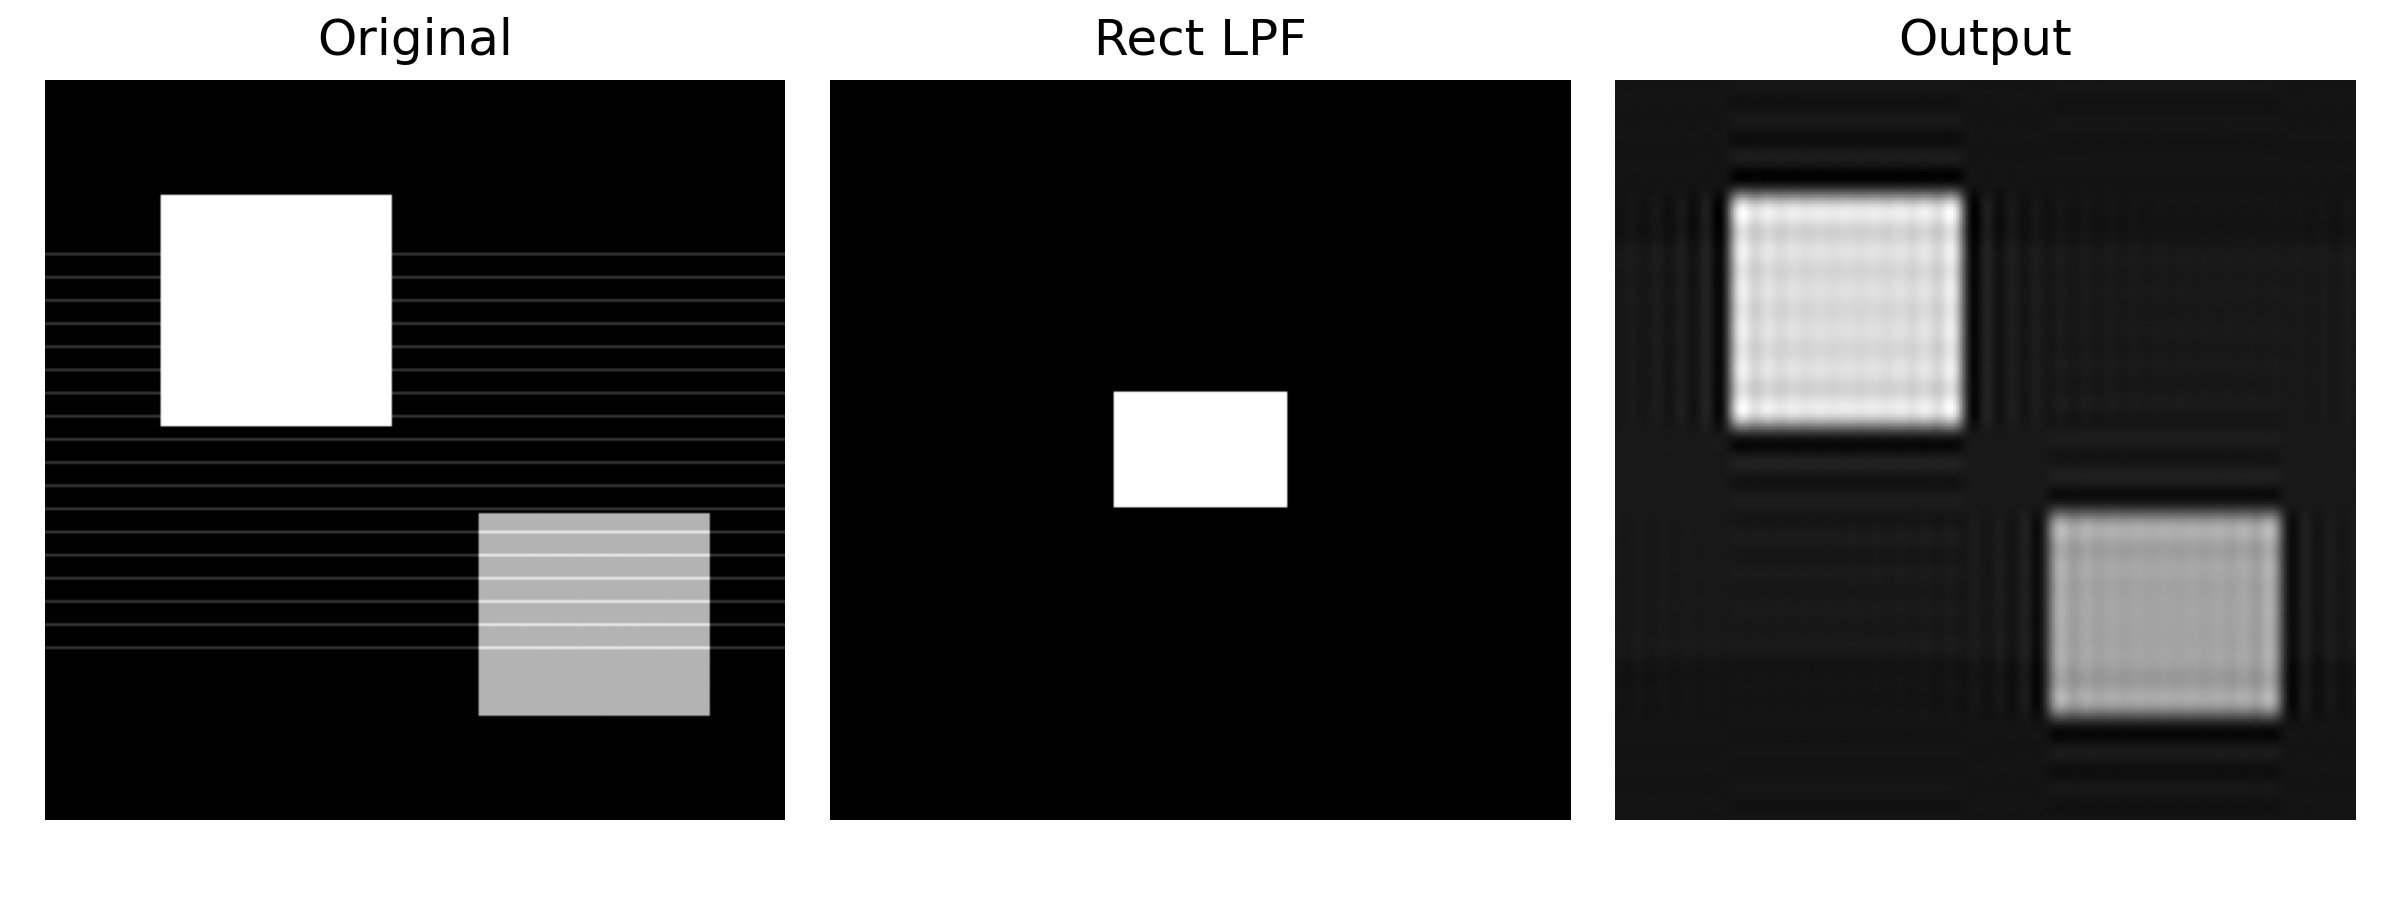
\includegraphics{plots/problem_3_rectangular.png}
			\caption{Low-pass rectangular support in the frequency domain and the corresponding output image.}
		\end{figure}
		
		\newpage
		
		\item Sketch the effect of convolution with a low-pass filter support over a disk in the frequency domain. What frequencies are missing from the output image? How does the image appear?\\
		
		\textbf{Solution.}
		For a filter with low-pass support over a disk in the frequency domain, the frequencies outside the disk are removed. Thus, the missing frequencies are the higher-frequency components outside the circular passband. The output image appears blurred, but now the smoothing is more uniform in all directions because the support is circular.
		
		\begin{figure}[H]
			\centering
			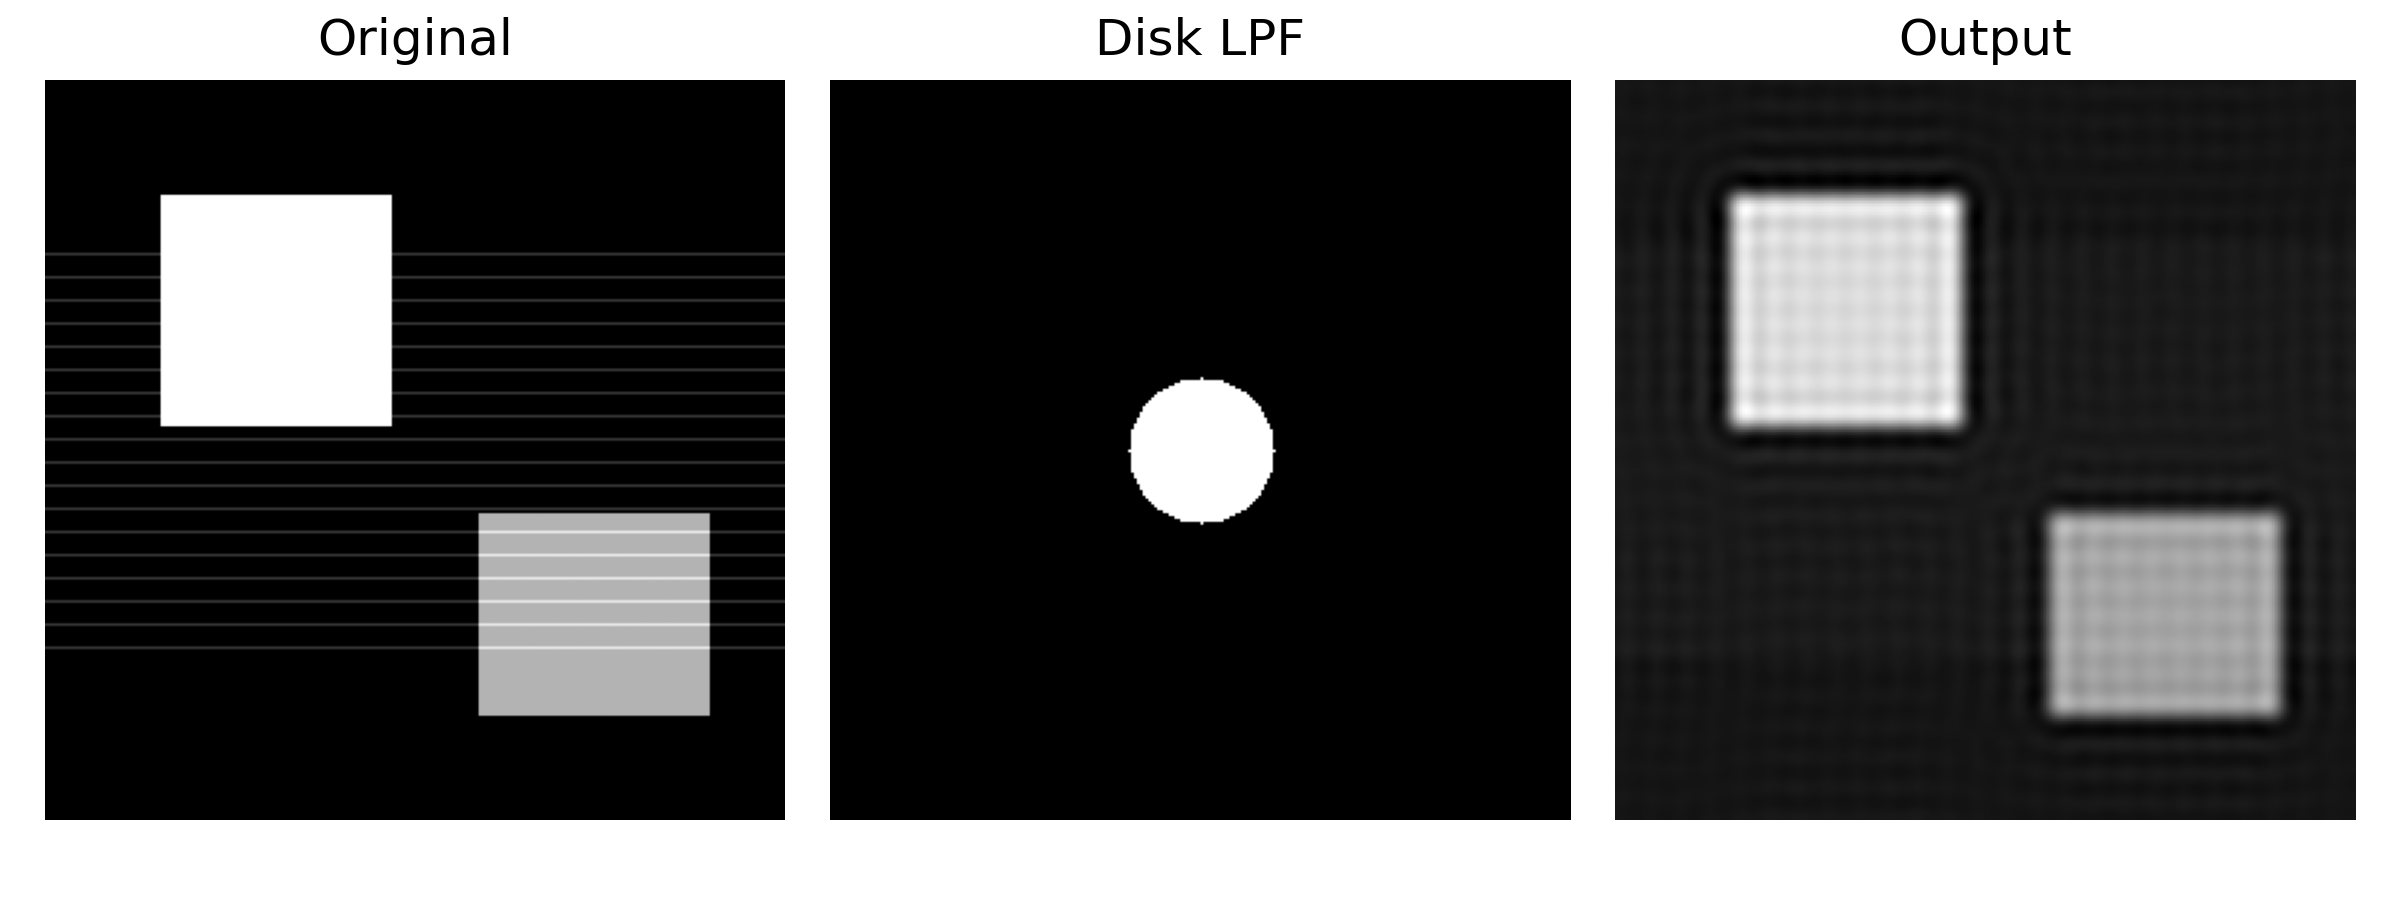
\includegraphics{plots/problem_3_disk.png}
			\caption{Low-pass disk support in the frequency domain and the corresponding output image.}
		\end{figure}
		
		\item For a filter with circular support, show that rotation of the input image does not remove frequency content.\\
		
		\textbf{Solution.}
		For a filter with circular support, rotation of the input image does not remove frequency content. The reason is that circular support is unchanged under rotation. Thus, rotating the input rotates the spectrum, but the same frequencies remain within the circular passband. Hence, the output is the same up to rotation.
		
		\begin{figure}[H]
			\centering
			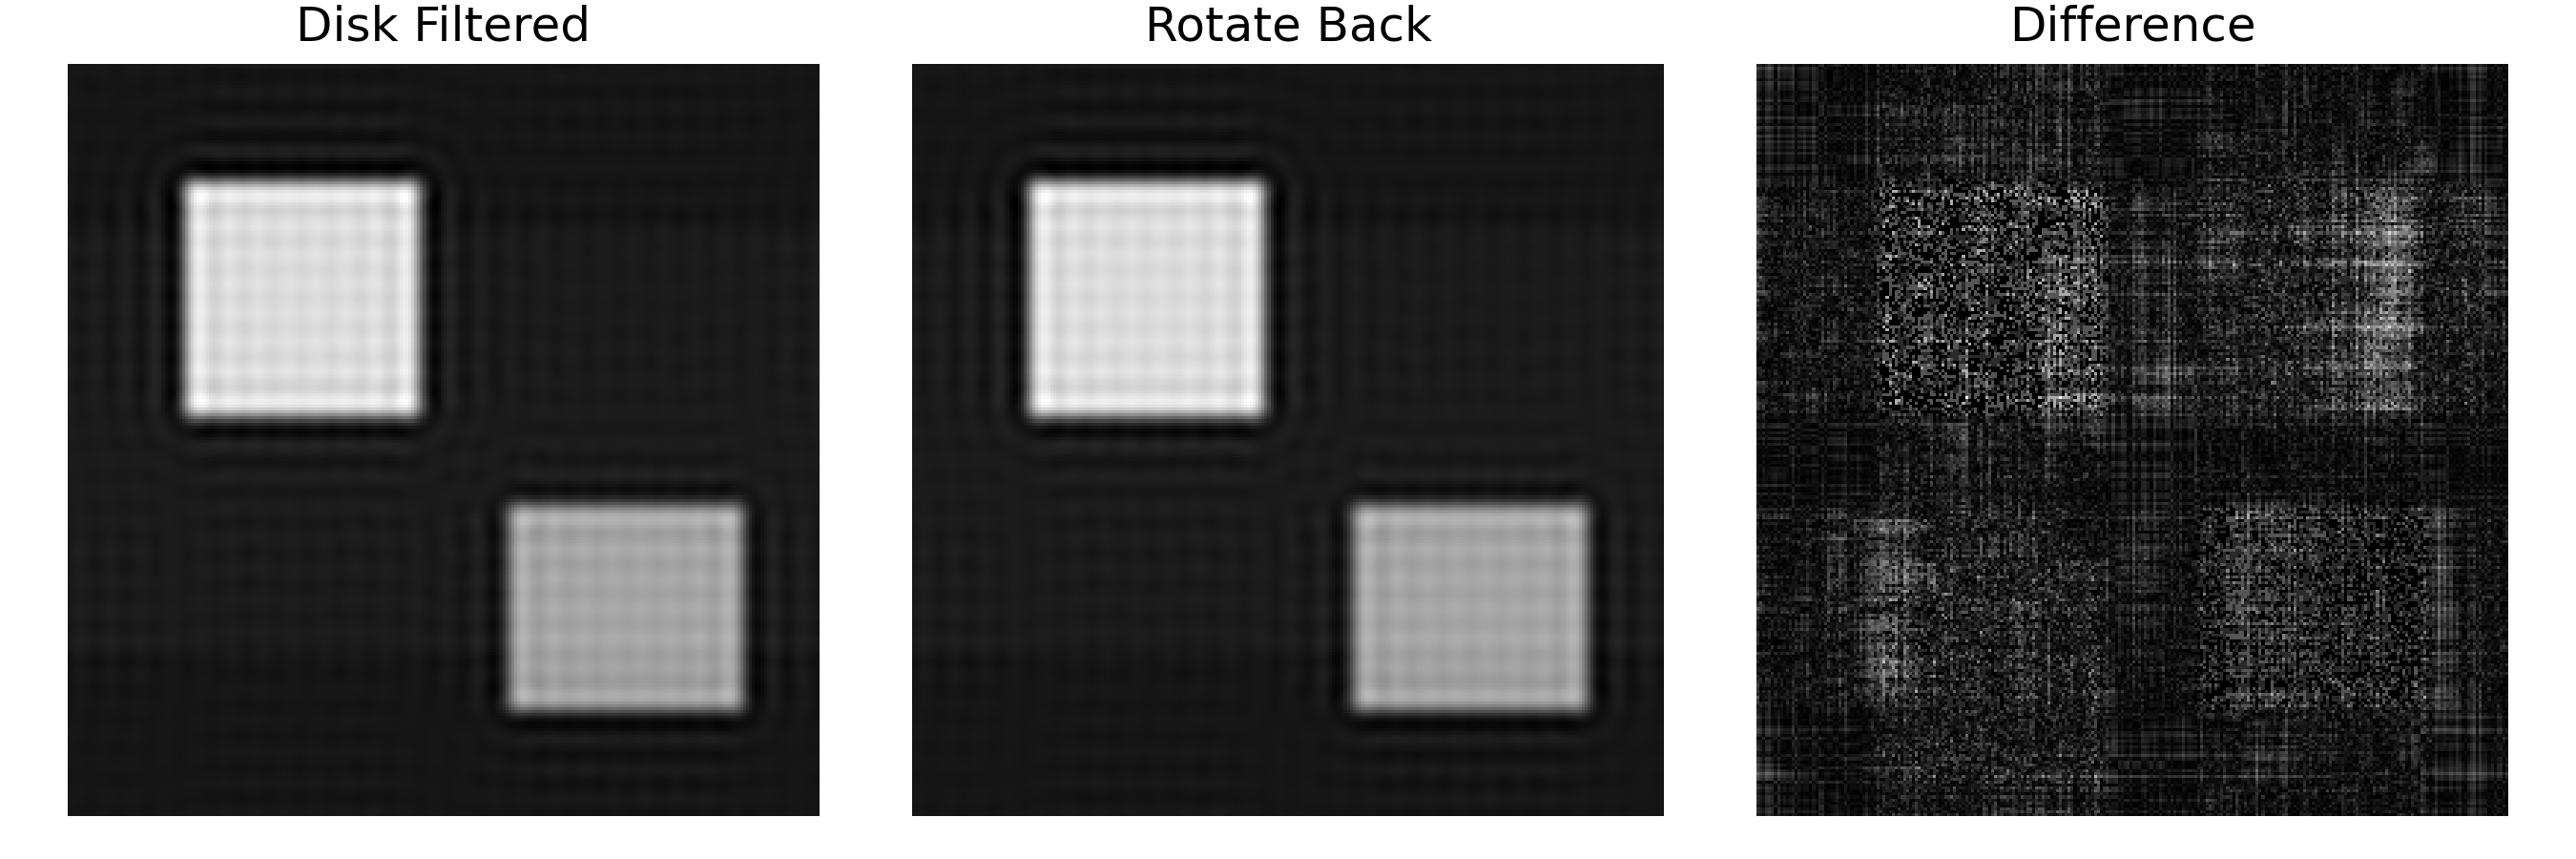
\includegraphics{plots/problem_3_rotation.png}
			\caption{Circular support: rotating the input and filtering yields the same result up to rotation.}
		\end{figure}
		
	\end{itemize}
	
	\newpage
	
	\begin{lstlisting}[language=Python]
	import os
	import numpy as np
	import matplotlib.pyplot as plt
	
	os.makedirs("plots", exist_ok=True)
	
	# --------------------------------------------------
	# Simple test image
	# --------------------------------------------------
	N = 256
	img = np.zeros((N, N))
	img[40:120, 40:120] = 1.0
	img[150:220, 150:230] = 0.7
	img[60:200:8, :] += 0.2
	img = np.clip(img, 0, 1)
	
	# --------------------------------------------------
	# Fourier transform
	# --------------------------------------------------
	F = np.fft.fftshift(np.fft.fft2(img))
	
	# Frequency grid
	u = np.arange(N) - N // 2
	v = np.arange(N) - N // 2
	U, V = np.meshgrid(u, v)
	
	# --------------------------------------------------
	# 1) Rectangular low-pass
	# --------------------------------------------------
	rect = np.zeros((N, N))
	rect[N//2-20:N//2+20, N//2-30:N//2+30] = 1
	
	F_rect = F * rect
	img_rect = np.real(np.fft.ifft2(np.fft.ifftshift(F_rect)))
	
	plt.figure(figsize=(8, 3))
	plt.subplot(1, 3, 1)
	plt.imshow(img, cmap="gray")
	plt.title("Original")
	plt.axis("off")
	
	plt.subplot(1, 3, 2)
	plt.imshow(rect, cmap="gray")
	plt.title("Rect LPF")
	plt.axis("off")
	
	plt.subplot(1, 3, 3)
	plt.imshow(img_rect, cmap="gray")
	plt.title("Output")
	plt.axis("off")
	
	plt.tight_layout()
	plt.savefig("plots/problem_3_rectangular.png", dpi=300)
	plt.close()
	
	# --------------------------------------------------
	# 2) Disk low-pass
	# --------------------------------------------------
	disk = ((U**2 + V**2) <= 25**2).astype(float)
	
	F_disk = F * disk
	img_disk = np.real(np.fft.ifft2(np.fft.ifftshift(F_disk)))
	
	plt.figure(figsize=(8, 3))
	plt.subplot(1, 3, 1)
	plt.imshow(img, cmap="gray")
	plt.title("Original")
	plt.axis("off")
	
	plt.subplot(1, 3, 2)
	plt.imshow(disk, cmap="gray")
	plt.title("Disk LPF")
	plt.axis("off")
	
	plt.subplot(1, 3, 3)
	plt.imshow(img_disk, cmap="gray")
	plt.title("Output")
	plt.axis("off")
	
	plt.tight_layout()
	plt.savefig("plots/problem_3_disk.png", dpi=300)
	plt.close()
	
	# --------------------------------------------------
	# 3) Circular support and rotation
	# --------------------------------------------------
	img_rot = np.rot90(img)
	
	F_rot = np.fft.fftshift(np.fft.fft2(img_rot))
	F_rot_disk = F_rot * disk
	img_rot_disk = np.real(np.fft.ifft2(np.fft.ifftshift(F_rot_disk)))
	
	# Rotate back to compare
	img_rot_disk_back = np.rot90(img_rot_disk, -1)
	
	plt.figure(figsize=(9, 3))
	plt.subplot(1, 3, 1)
	plt.imshow(img_disk, cmap="gray")
	plt.title("Disk Filtered")
	plt.axis("off")
	
	plt.subplot(1, 3, 2)
	plt.imshow(img_rot_disk_back, cmap="gray")
	plt.title("Rotate Back")
	plt.axis("off")
	
	plt.subplot(1, 3, 3)
	plt.imshow(np.abs(img_disk - img_rot_disk_back), cmap="gray")
	plt.title("Difference")
	plt.axis("off")
	
	plt.tight_layout()
	plt.savefig("plots/problem_3_rotation.png", dpi=300)
	plt.close()
	
	print("Saved:")
	print("plots/problem_3_rectangular.png")
	print("plots/problem_3_disk.png")
	print("plots/problem_3_rotation.png")
	\end{lstlisting}
	
	
\end{document}